\documentclass[12pt,a4paper]{article}
\usepackage{amsmath}
\usepackage{mathtext}
\usepackage{icomma}
\usepackage{amsfonts}
\usepackage{amssymb}
\usepackage[utf8]{inputenc}
\usepackage[T1,T2A]{fontenc}
\usepackage[english, russian]{babel}
\usepackage{graphicx}
\usepackage[left=2cm,right=2cm,top=2cm,bottom=2cm]{geometry}
\usepackage{calc}
\usepackage{wrapfig}
\usepackage{setspace}
\usepackage{indentfirst}
\usepackage{subfigure}
\usepackage[table,xcdraw]{xcolor}
\usepackage{float}

\title{Отчет о выполнении лабораторной работы 3.2.1\\
Изучение плазмы газового разряда в неоне}

\author{Исламов Сардор, группа Б02-111}

\begin{document}
\maketitle

\subparagraph*{Аннотация.} В ходе работы снята вольт-амперная характеристика тлеющего разряда и зондовые характеристики при разных токах разряда.
По результатам измерений рассчитаны концентрация и температура электронов в плазме, плазменная частота, поляризационная длина, дебаевский радиус экранирования и степень ионизации.

\subsection*{Теоретическое введение}
\subparagraph*{Плазма.}В ионизированном газе поле ионов <<экранируется>> электронами. 
Для поля $\mathbf{E}$ и плотности $\rho$ электрического заряда
\[\text{div}~\mathbf{E} = 4 \pi \rho,\]
а с учётом сферической симметрии и $\mathbf{E} = -\text{grad}~\varphi$:
\begin{equation}
    \dfrac{d^2 \varphi}{dr^2}+\dfrac{2}{r}\dfrac{d\varphi}{dr}=-4\pi \rho.
\end{equation}
Плотности заряда электронов и ионов (которые мы считаем бесконечно тяжёлыми и поэтому неподвижными)
\begin{equation}
    \begin{array}{c}
        \rho_e = -ne \cdot \exp\left(\dfrac{e\varphi}{kT_e}\right),\\
        \rho_i = ne.
    \end{array}
\end{equation}
Тогда из $(1)$ в предположении $\dfrac{e\varphi}{kT_e} \ll 1$ получим
\begin{equation}
    \varphi = \dfrac{Ze}{r}e^{-r/r_D},
\end{equation}
где $r_D = \sqrt{\dfrac{kT_e}{4\pi n e^2}}$ -- радиус Дебая. 
Среднее число ионов в сфере такого радиуса 
\begin{equation}
    N_D = n\dfrac{4}{3}\pi r_D^2.
\end{equation}

\begin{wrapfigure}{r}{0.3\linewidth}
    \centering
    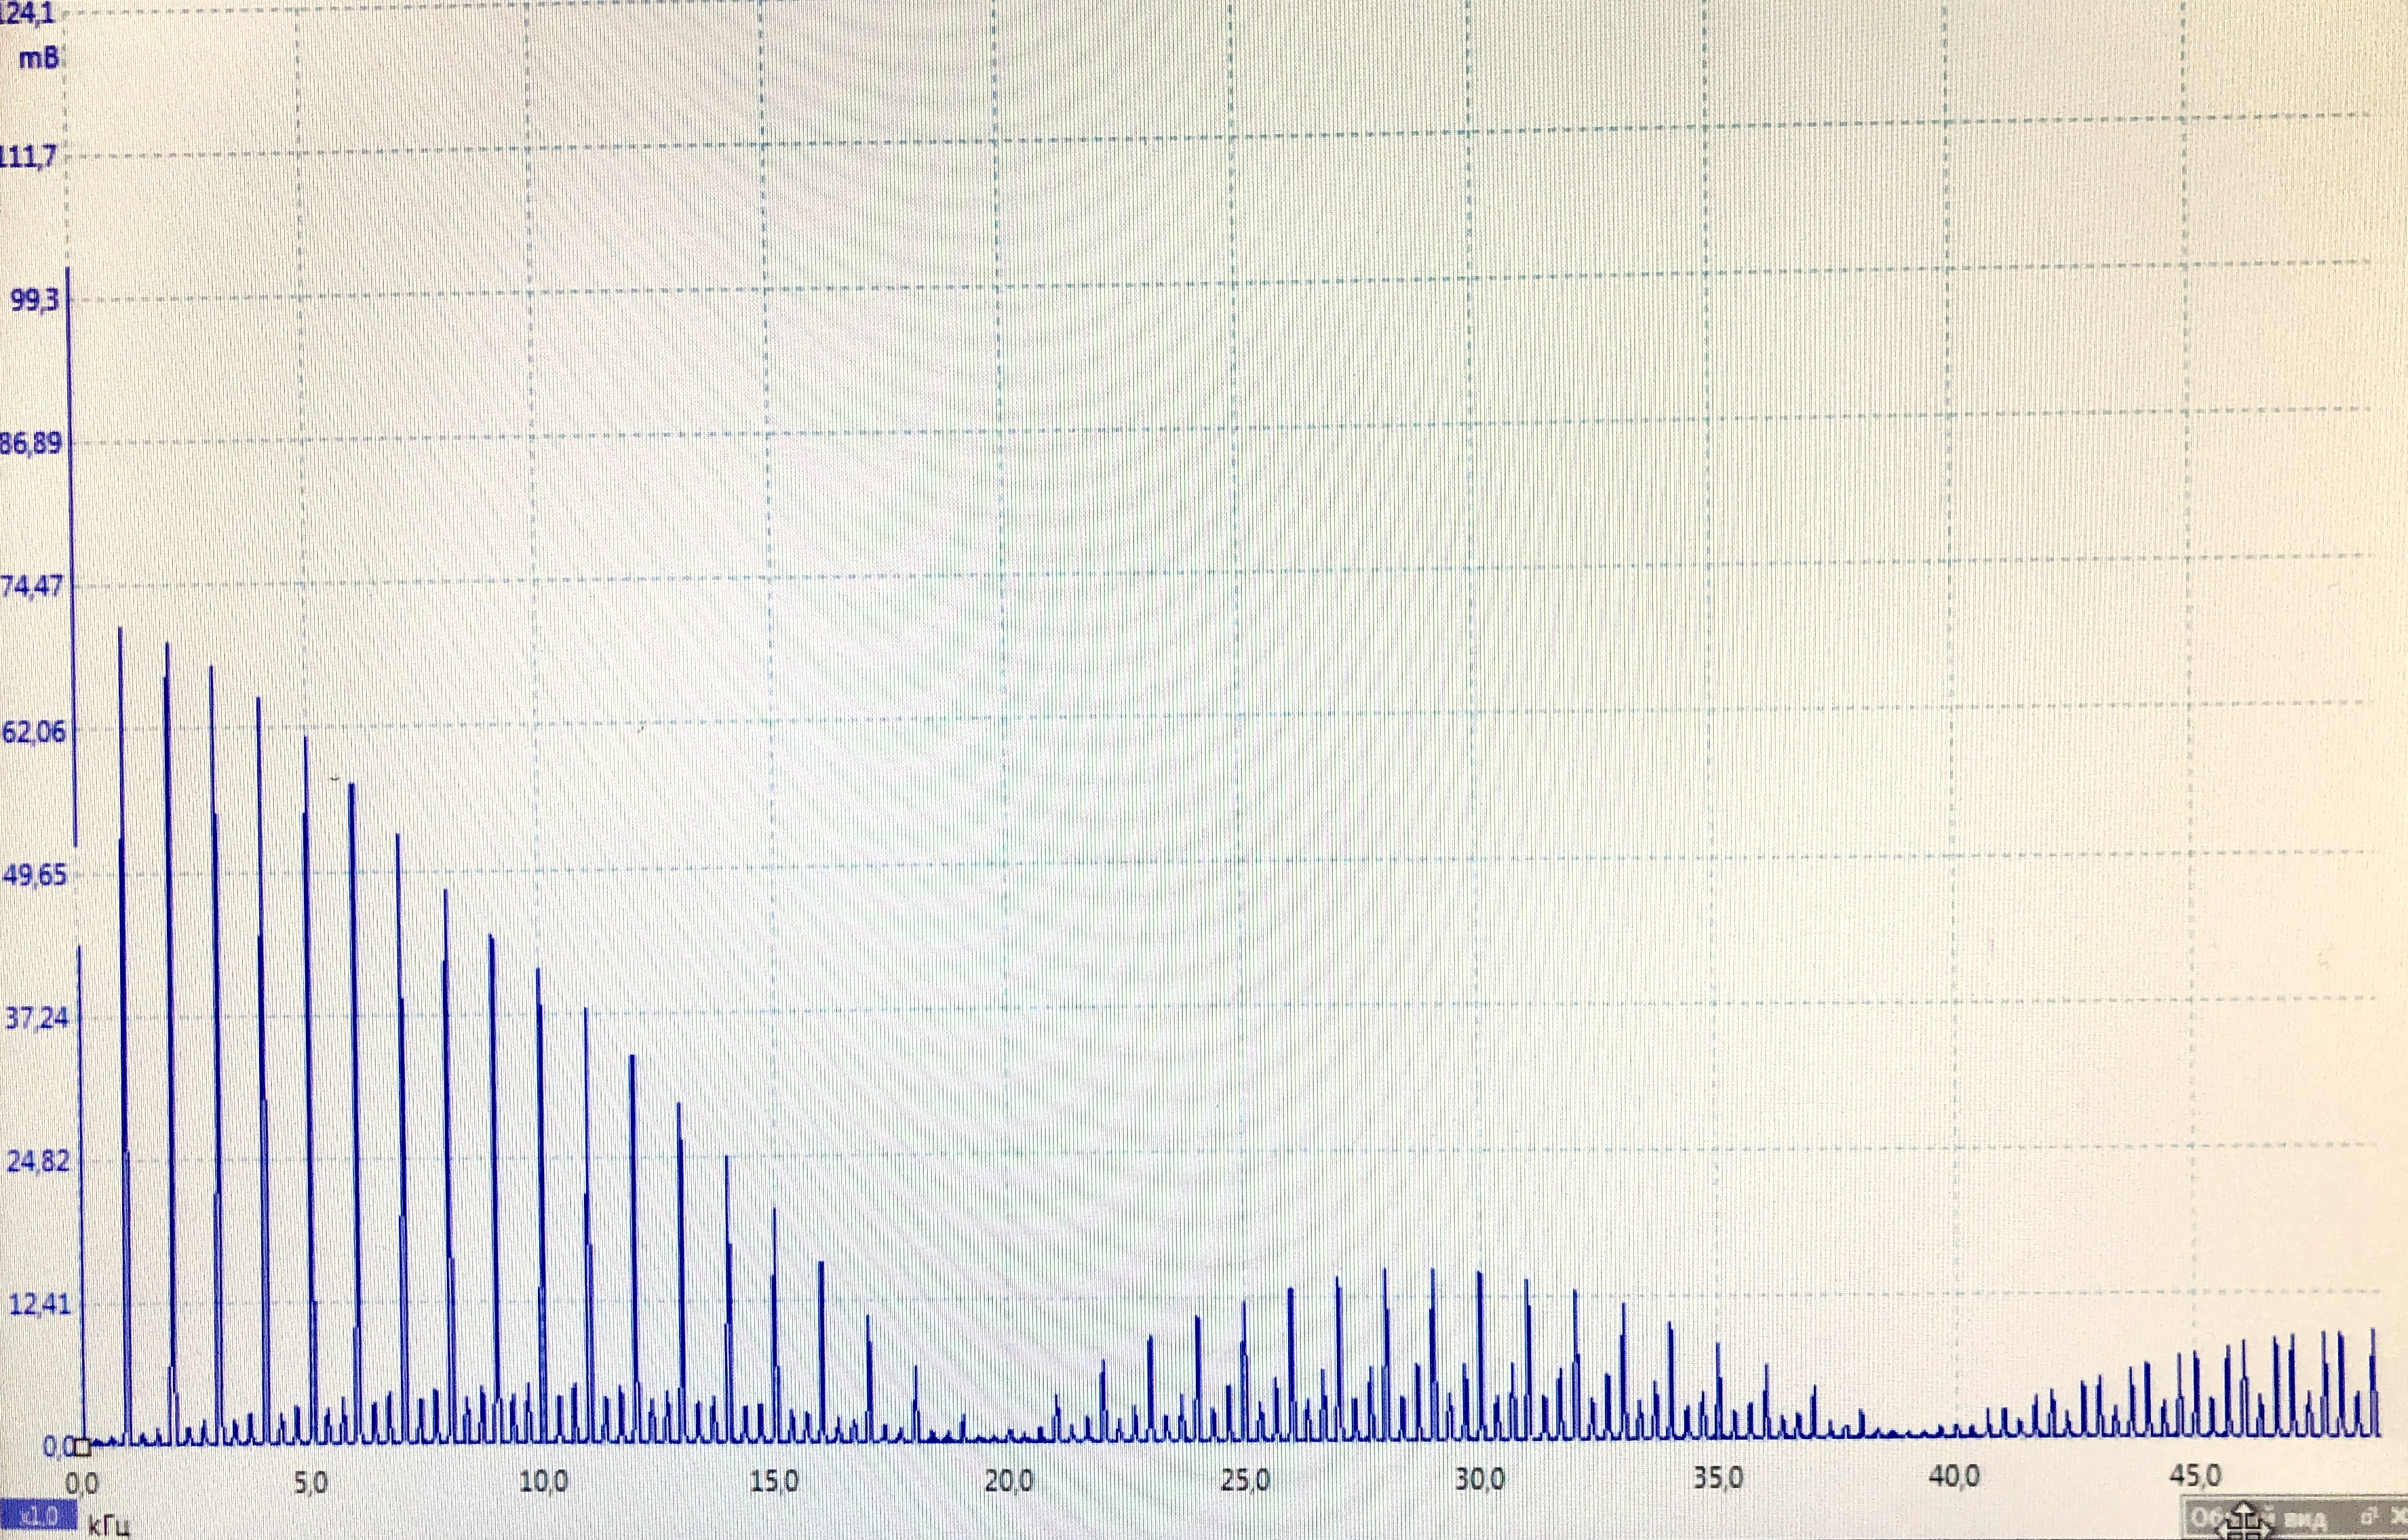
\includegraphics[width=0.6\linewidth]{pics/1.png}
    \caption{\small{Параллелепипед с плотностью $n$}}
\end{wrapfigure}  

Теперь выделим параллелепипед с плотностью $n$ электронов (рис. 1), сместим их на $x$. 
Возникнут поверхностные заряды $\sigma = nex$, поле от которых будет придавать электронам ускорение:
\[\dfrac{d^2x}{dt^2}=-\dfrac{eE}{m}=-\dfrac{4\pi n e^2}{m}x.\]

Отсюда получаем плазменную (ленгмюровскую) частоту колебаний электронов:
\begin{equation}
    \omega_p = \sqrt{\dfrac{4\pi ne^2}{m}}.
\end{equation}

\subparagraph*{Одиночный зонд.}
При внесении в плазму уединённого проводника -- зонда -- с потенциалом, изначально равным потенциалу точки плазмы, в которую его помещают, на него поступают токи электроннов и ионов:
\begin{equation}
        I_{e0} = \dfrac{n \langle v_e \rangle}{4}eS,\quad I_{i0} = \dfrac{n \langle v_i \rangle}{4}eS,
\end{equation}
где $\langle v_e \rangle$ и $\langle v_i \rangle$ -- средние скорости электронов и ионов, $S$ -- площадь зонда, $n$ -- плотность электронов и ионов. 
Скорости электронов много больше скорости ионов, поэтому $I_{i0} \ll I_{e0}$. 
Зонд будет заряжаться до некоторого равновестного напряжения $-U_f$ -- плавающего потенциала.\\

\begin{wrapfigure}{r}{0.4\linewidth}
    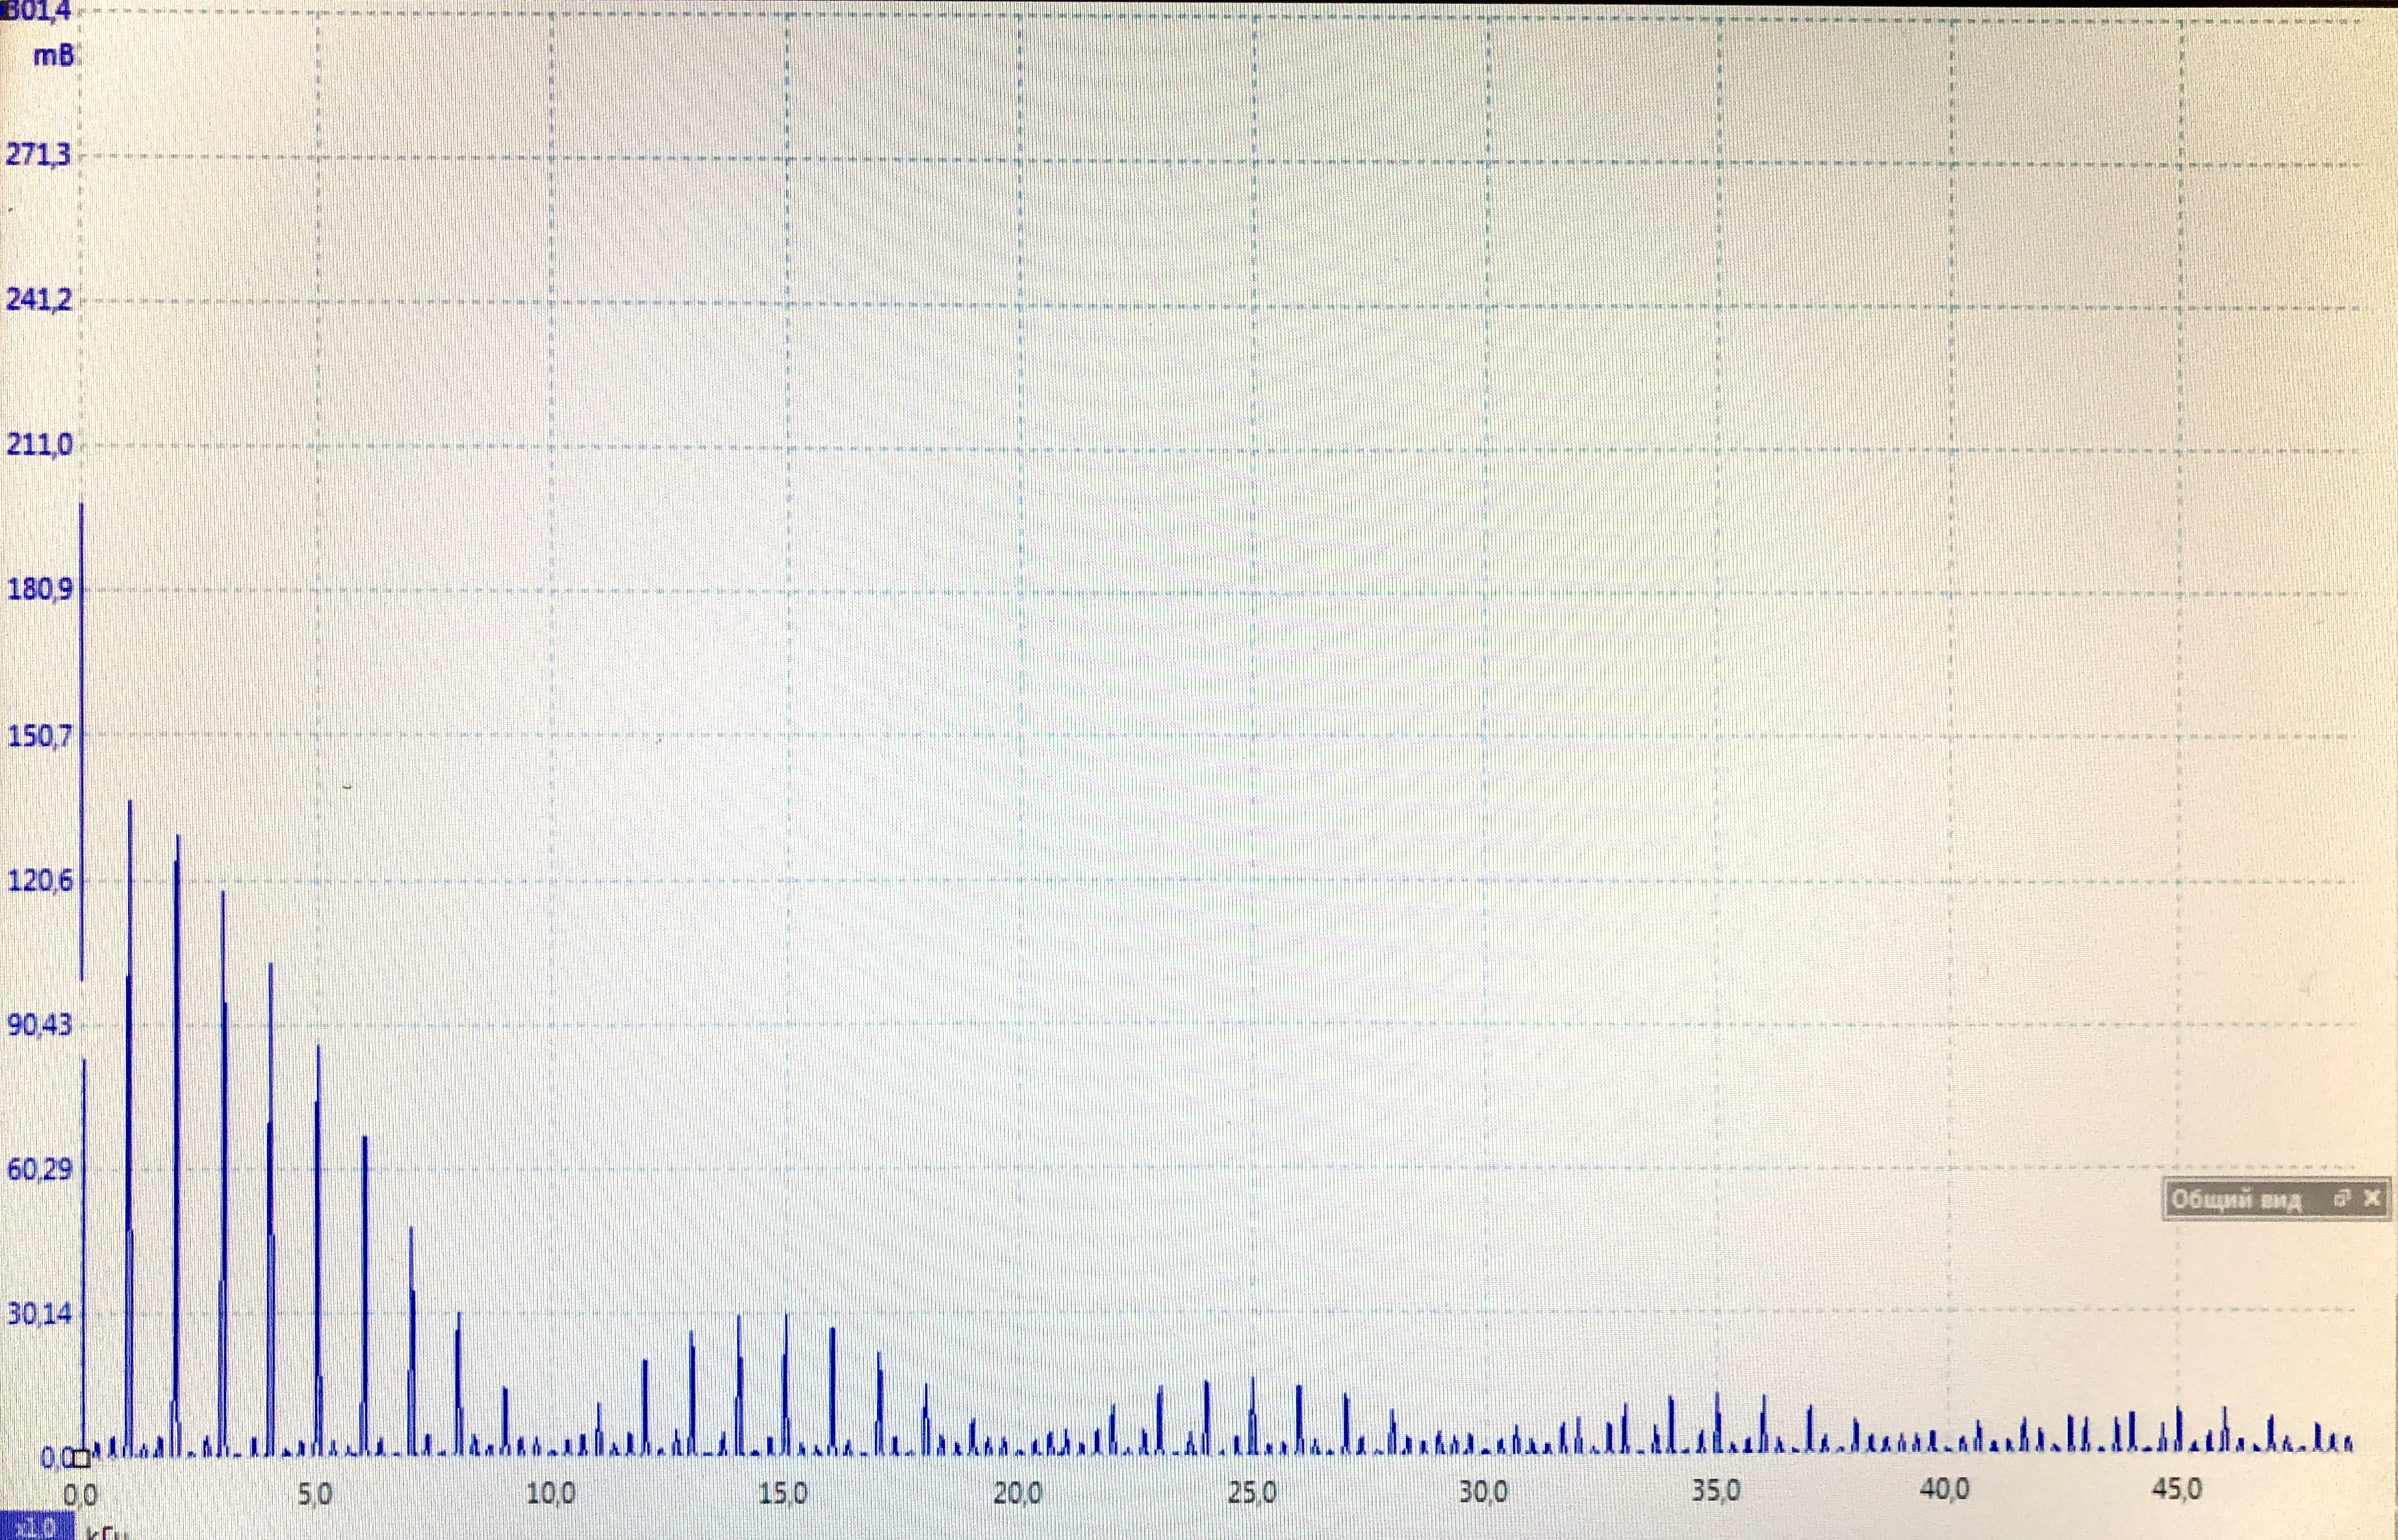
\includegraphics[width=\linewidth]{pics/2.png}
    \caption{\small{Вольт-амперная характеристика одиночного зонда}}
\end{wrapfigure}  

В равновесии ионный ток мало меняется, а электронный имеет вид
\[I_e = I_0 \exp\left( -\dfrac{eU_f}{kT_e} \right).\]

Будем подавать потенциал $U_\text{з}$ на зонд и снимать значение зондового тока $I_\text{з}$. 
Максимальное значение тока $I_{e\text{н}}$ -- электронный ток насыщения, а минимальное $I_{i\text{н}}$ -- ионный ток насыщения. 
Значение из эмпирической формулы Бомона:
\begin{equation}
    I_{i\text{н}} = 0.4 neS \sqrt{\dfrac{2kT_e}{m_i}}.
\end{equation}

\subparagraph*{Двойной зонд.}
Двойной зонд -- система из двух одинаковых зондов, расположенных на небольшом расстоянии друг от друга, между которыми создаётся разность потенциалов, меньшая $U_f$. 
Рассчитаем ток между ними вблизи $I=0$. 
При небольших разностях потенциалов ионные токи на оба зонда близки к току насыщения и компенсируют друг друга, а значит величина результирующего тока полностью связана с разностью электронных токов. 
Пусть потенциалы на зондах
\[U_1 = -U_f + \Delta U_1,\]

\[U_2 = -U_f + \Delta U_2.\]

Между зондами $U = U_2 - U_1 = \Delta U_2 - \Delta U_1$.
Через первый электрод
\begin{equation}
    I_1 = I_{iн} + I_{e1} = I_{iн} - \dfrac{1}{4}neS\langle v_e\rangle \exp\left(-\dfrac{eU_f}{kT_e}\right)\exp\left(\dfrac{e\Delta U_1}{kT_e}\right)=I_{iн}\left(1 - \exp\left( \dfrac{e\Delta U_1}{kT_e} \right)\right).
\end{equation}

Аналогично через второй получим
\begin{equation}
    I_2 = I_{iн}\left(1 - \exp\left( \dfrac{e\Delta U_2}{kT_e} \right)\right)
\end{equation}
  
Из $(7)$ и $(8)$ с учётом последовательного соединение зондов ($I_1 = -I_2 = I)$:
\[\Delta U_1= \dfrac{kT_e}{e}\text{ln}\left(1 - \dfrac{I}{I_{iн}}\right)\]
\[\Delta U_2= \dfrac{kT_e}{e}\text{ln}\left(1 + \dfrac{I}{I_{iн}}\right)\]

\begin{wrapfigure}{l}{0.4\linewidth}
    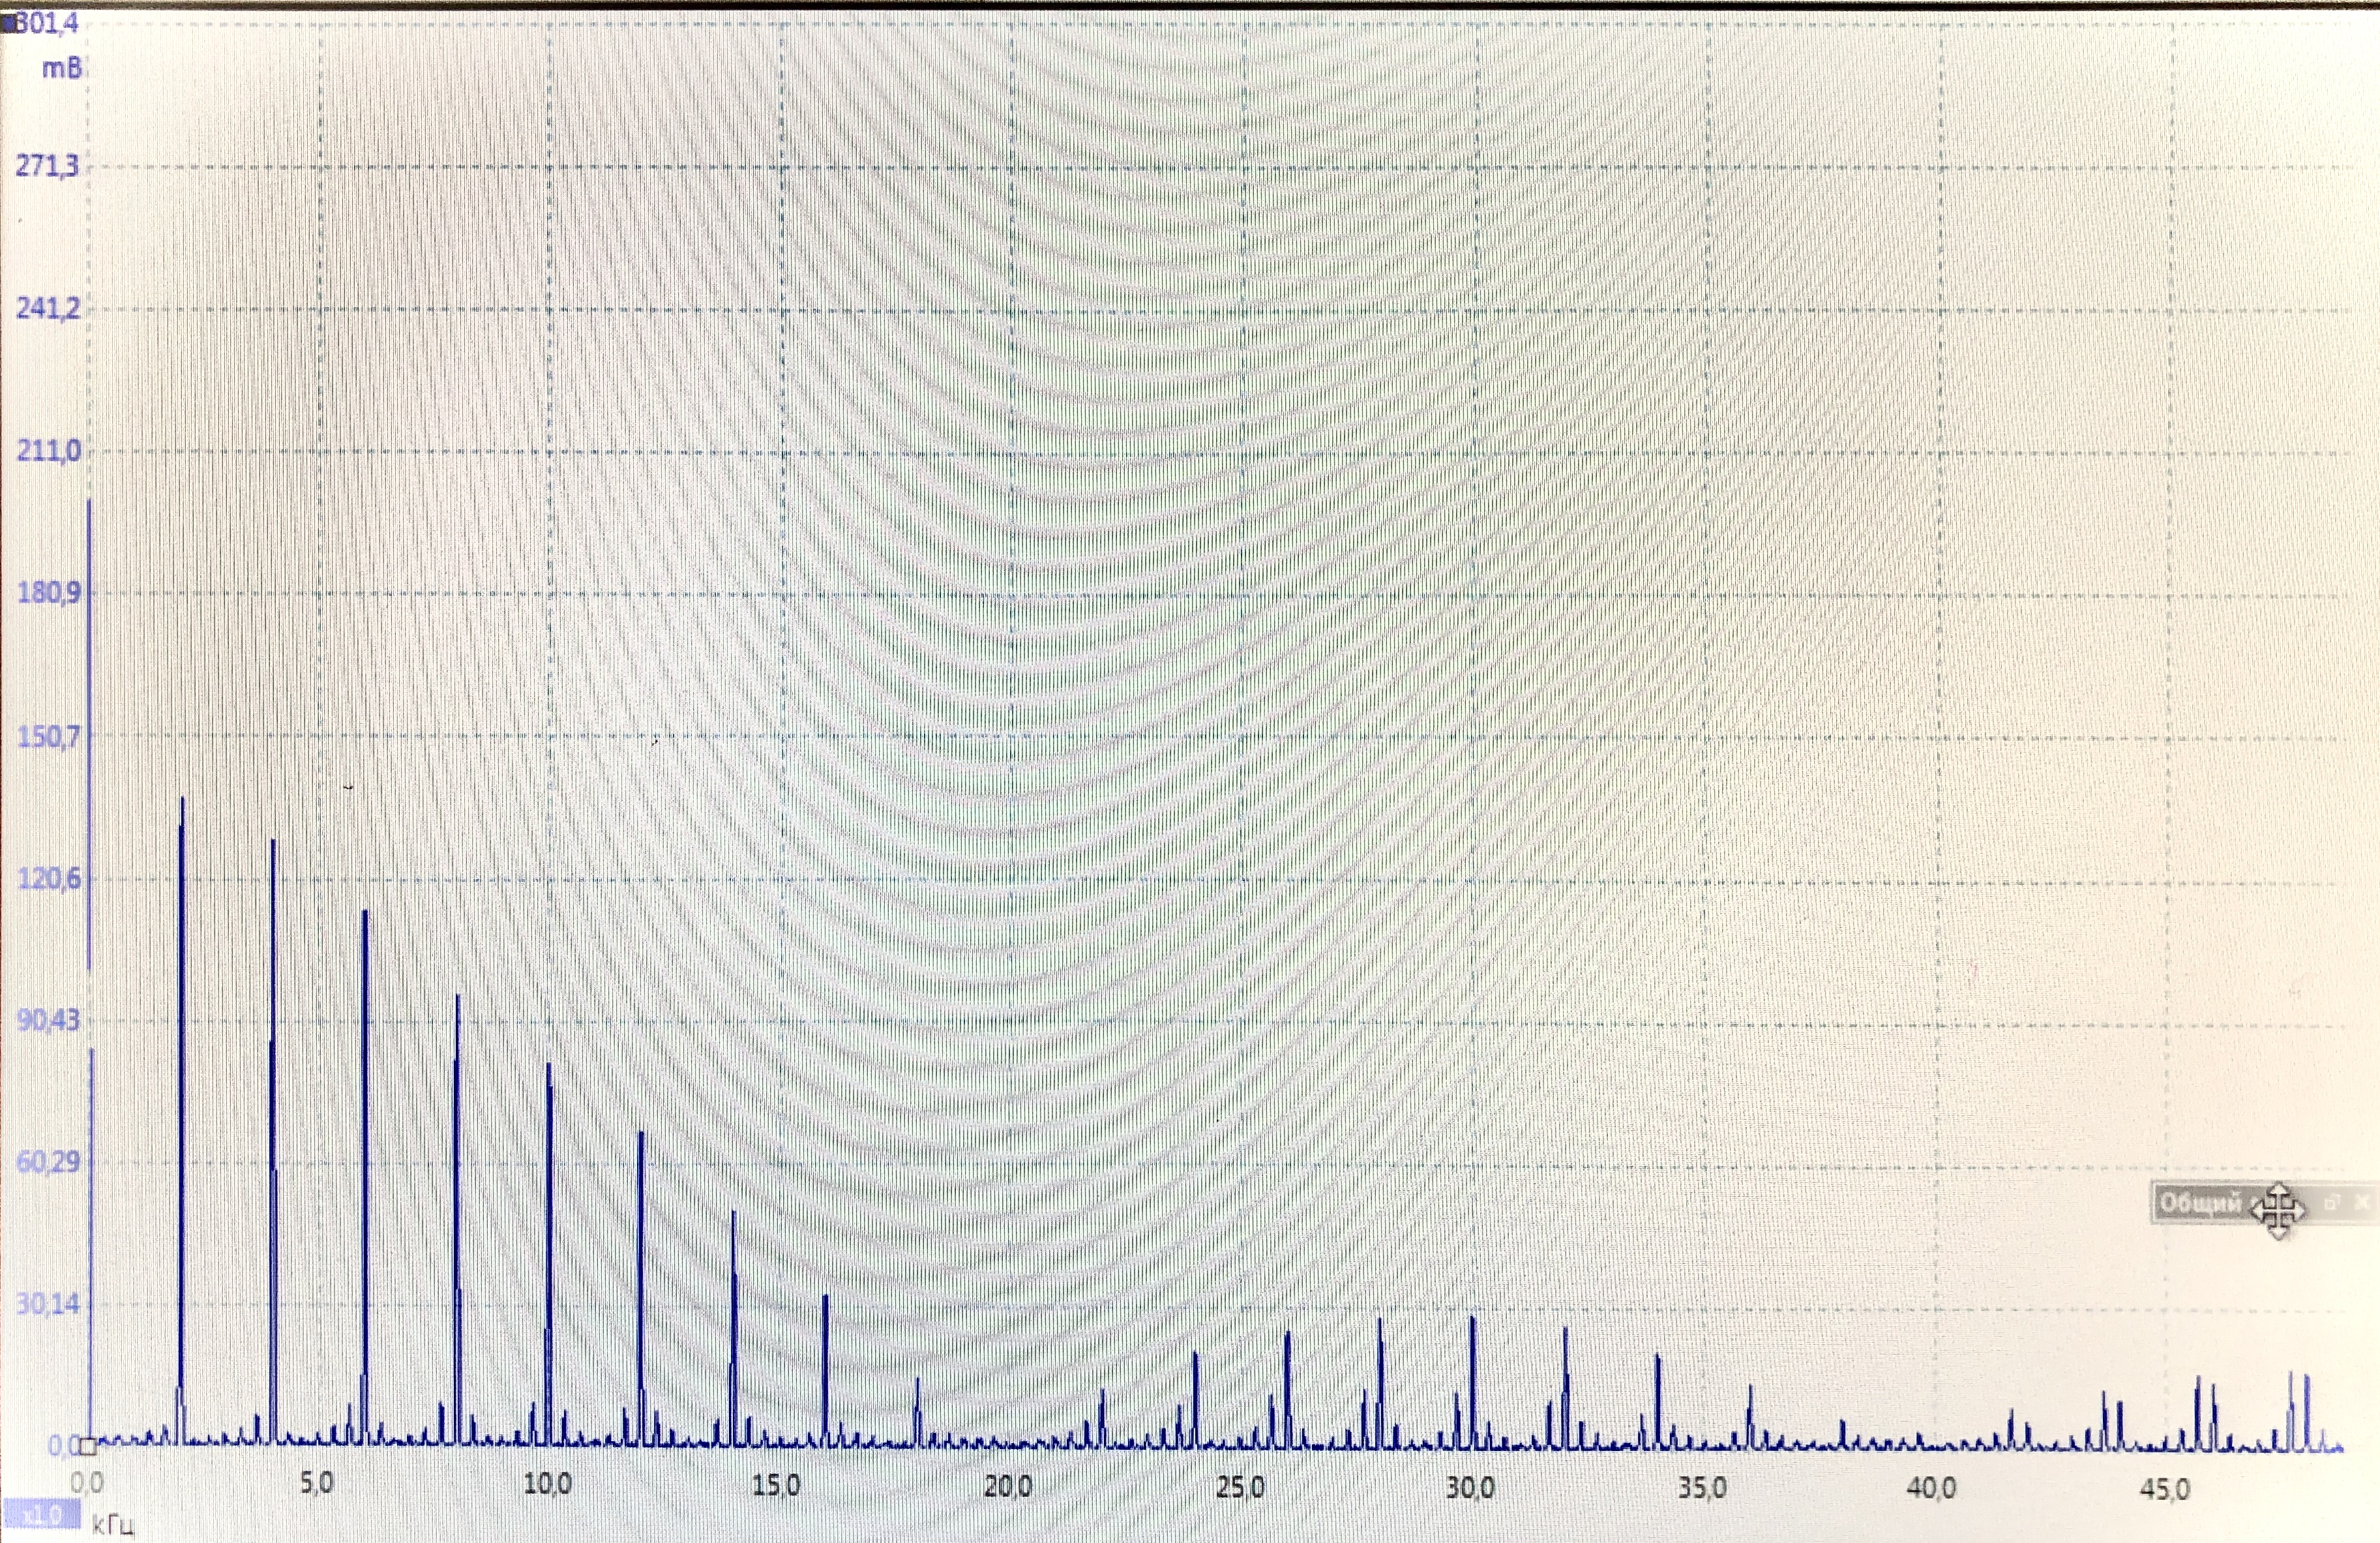
\includegraphics[width=\linewidth]{pics/3.png}
    \caption{\small{Вольт-амперная характеристика двойного зонда}}
\end{wrapfigure}

Тогда итоговые формулы для разности потенциалов и тока

\begin{equation}
    U = \frac{kT_e}{e}\text{ln}\frac{1 - I/I_{iн}}{1 + I/I_{iн}}, \quad
    I = I_{iн} \tanh\dfrac{eU}{2kT_e}.
\end{equation}

Реальная зависимость выглядит несколько иначе и описывается формулой 

\begin{equation}
    I = I_{iн} \tanh\frac{eU}{2kT_e} + AU.
\end{equation}
Из этой формулы можно найти формулу для $T_e$: для $U=0$ мы найдём $I_{iн}$, продифференцируем в точке $U=0$ и с учётом $\tanh \alpha \approx \alpha$ при малых $\alpha$ и $A\rightarrow 0$ получим:
\begin{equation}
    kT_e = \dfrac{1}{2}\dfrac{eI_{iн}}{\dfrac{dI}{dU}|_{U=0}}.
\end{equation}

\subsection*{Экспериментальная установка}
Схема установки для исследования плазмы газового разряда в неоне представлена на рис. 1. 
Стеклянная газоразрядная трубка имеет холодный (ненагреваемый) полый катод, три анода и геттерный узел - стеклянный баллон, на внутреннюю поверхность которого напылена газопоглощающая плёнка (геттер). 
Трубка наполнена изотопом неона ${}^{22}$Ne при давлении 2 мм рт. ст. 
Катод и один из анодов (I или II) с помощью переключателя $П_1$ подключаются через балластный резистор $R_{\sigma}(\sim 450$ кОм $)$ к регулируемому высоковольтному источнику питания (ВИП) с выходным напряжением до 5 кВ.
\begin{figure}[H]
    \centering
    \includegraphics[width=0.7\linewidth]{pics/scheme.png}
    \caption{Схема установки для исследования газового разряда}
\end{figure}

При подключении к ВИП анода-I между ним и катодом возникает газовый разряд. 
Ток разряда измеряется миллиамперметром $A_{1}$, а падение напряжения на разрядной трубке - цифровым вольтметром $V_{1}$ (мультиметром GDM), подключённым к трубке через высокоомный (25 МОм) делитель напряжения с коэффициентом $\left(R_{1}+R_{2}\right) / R_{2}=10$.

При подключении к ВИП анода-II разряд возникает в пространстве между катодом и анодом-II, где находится двойной зонд, используемый для диагностики плазмы положительного столба.

Зонды изготовлены из молибденовой проволоки диаметром $d=0.2$ мм и имеют длину $l=5.2$ мм. 
Они подключены к источнику питания GPS через потенциометр $R$. 
Переключатель $\Pi_{2}$ позволяет изменять полярность напряжения на зондах. 
Величина напряжения на зондах изменяется с помощью дискретного переключателя «$V$» выходного напряжения источника питания и потенциометра $R$, а измеряется цифровым вольтметром $V_{2}(\mathrm{GDM})$. 
Для измерения зондового тока используется мультиметр $A_{2}(\mathrm{GDM})$. 
Анод-III в нашей работе не используется. 

\subsection*{Результаты измерений и обработка данных}
Для начала, плавно увеличивая напряжение на ВИП определим напряжение зажигания разряда $U_{заж} = 228В$.

Теперь снимем зависимость напряжения разряда $U_p$ от его тока $I_p$ как при его увеличении, так и при убывании (табл. 1).
\begin{table}[H]
    \centering
    \begin{tabular}[]{|c|c|c|c|c|c|c|c|c|c|c|c|c|c|c|}
        \hline
        $I_p$, дел &125&115&105&95&85&75&65&55&45&35&25&14\\
        \hline
        $U_p\downarrow$, В &24.34&24.47&24.85&25.49&26.54&27.45&26.70&28.48&30.49&32.95&33.80&34.85\\
        \hline
        $U_p\uparrow$, В &24.27&24.42&24.78&25.42&26.46&27.40&26.66&28.40&30.69&32.96&33.83&34.84\\
        \hline
    \end{tabular}
    \caption{Вольт-амперная характеристика разряда}
\end{table}

Изобразим полученные данные на графике (рис. 5)
\begin{figure}[H]
    \centering
    \includegraphics[width=0.9\linewidth]{pics/Ip_Up.eps}
    \caption{ВАХ рязряда}
\end{figure}
Максималльное дифференциальное сопротивлние заряда $R_{диф} = (5.9 \pm 0.2) \cdot 10^3$ Ом 
 
4) $GPS :U_2=25, GDM: U=24.98$

Проведем серию измерений для вольт-амперной характеристики двойного зонда при различных разрядных токах (табл. 2).  
\begin{table}[H]
    \centering
    \resizebox{\textwidth}{!}{
    \begin{tabular}[]{|c|c|c|c|c|c|c|c|c|c|c|c|}
        \hline
        \multicolumn{12}{|c|}{$I_p = 5$ мА} \\
        \hline
        $U_з$, В, &24.958  & 22.011 & 19.046 & 15.860 & 13.170 & 10.000 & 8.088  & 5.962  & 3.9183 & 2.1389 & 0.6032 \\
        \hline
        $I_з$, мкА &107.91  & 104.46 & 101.80 & 98.96  & 94.37  & 85.33  & 76.10  & 64.40  & 49.85  & 35.11  & 21.29  \\
        \hline
        $-U_з$, В, &0.5530 & 2.0379 & 4.0678 & 6.091  & 8.044  & 9.971  & 13.028 & 16.000 & 19.148 & 22.083 & 24.964 \\
        \hline
        $-I_з$, мкА &9.01  & 33.30  & 51.12  & 65.72  & 77.45  & 87.38  & 98.40  & 105.13 & 109.91 & 113.03 & 115.68 \\ 
        \hline
        \multicolumn{12}{|c|}{$I_p = 3$ мА} \\
        \hline
        $U_з$, В, &25.045 & 22.088 & 19.035 & 16.232 & 13.060 & 10.138 & 8.112  & 5.965  & 3.9684 & 2.0783 & 0.6441 \\
        \hline
        $I_з$, мкА &58.00  & 56.39  & 54.73  & 53.11  & 50.58  & 46.46  & 41.64  & 34.58  & 25.83  & 15.91  & 6.96   \\
        \hline
        $-U_з$, В, &0.6429 & 2.0515 & 4.0726 & 6.000  & 8.005  & 9.999  & 13.047 & 16.156 & 18.909 & 22.112 & 24.988 \\
        \hline
        $-I_з$, мкА &5.03   & 14.23  & 25.45  & 34.30  & 41.69  & 47.12  & 52.38  & 55.17  & 56.92  & 58.73  & 60.37 \\
        \hline
        \multicolumn{12}{|c|}{$I_p = 1.5$ мА} \\
        \hline
        $U_з$, В, &24.991 & 21.953 & 19.000 & 16.032 & 13.161 & 10.042 & 7.944  & 5.955  & 3.9200 & 1.9521 & 0.5289 \\
        \hline
        $I_з$, мкА &27.61  & 26.64  & 25.73  & 24.79  & 23.63  & 21.52  & 19.13  & 15.97  & 11.71  & 6.39   & 2.18   \\
        \hline
        $-U_з$, В, &0.5345 & 2.0794 & 4.1773 & 6.079  & 7.989  & 10.249 & 13.350 & 16.303 & 18.987 & 22.242 & 24.967 \\
        \hline
        $-I_з$, мкА &1.81   & 6.29   & 12.01  & 16.23  & 19.60  & 22.46  & 24.75  & 26.07  & 26.96  & 28.01  & 28.90 \\
        \hline
    \end{tabular}}
    \caption{Зондовые характеристики при разных токах}
    \begin{flushright}
        \includegraphics[width=0.2\linewidth]{pics/signa.jpeg}
    \end{flushright}
\end{table}

Теперь отобразим данные на графиках и определим $I_{iн}$ и производную в нуле.

\begin{figure}[H]
    \centering
    \includegraphics[width=0.7\linewidth]{pics/UI1.eps}
    \caption{ВАХ двойного зонда при $I_p = 5$ мА}
\end{figure}

\begin{figure}[H]
    % \centering
    \subfigure[ВАХ двойного зонда при $I_p = 3$ мА]{
        \begin{minipage}{0.5\linewidth}
            \centering
            \includegraphics[width=\linewidth]{pics/UI2.eps}
        \end{minipage}
    }
    \subfigure[ВАХ двойного зонда при $I_p = 1.5$ мА]{
        \begin{minipage}{0.5\linewidth}
            \centering
            \includegraphics[width=\linewidth]{pics/UI3.eps}
        \end{minipage}
    }
\end{figure}

Также изобразим все ВАХ на одном графике (рис. 7)

\begin{figure}[H]
    \centering
    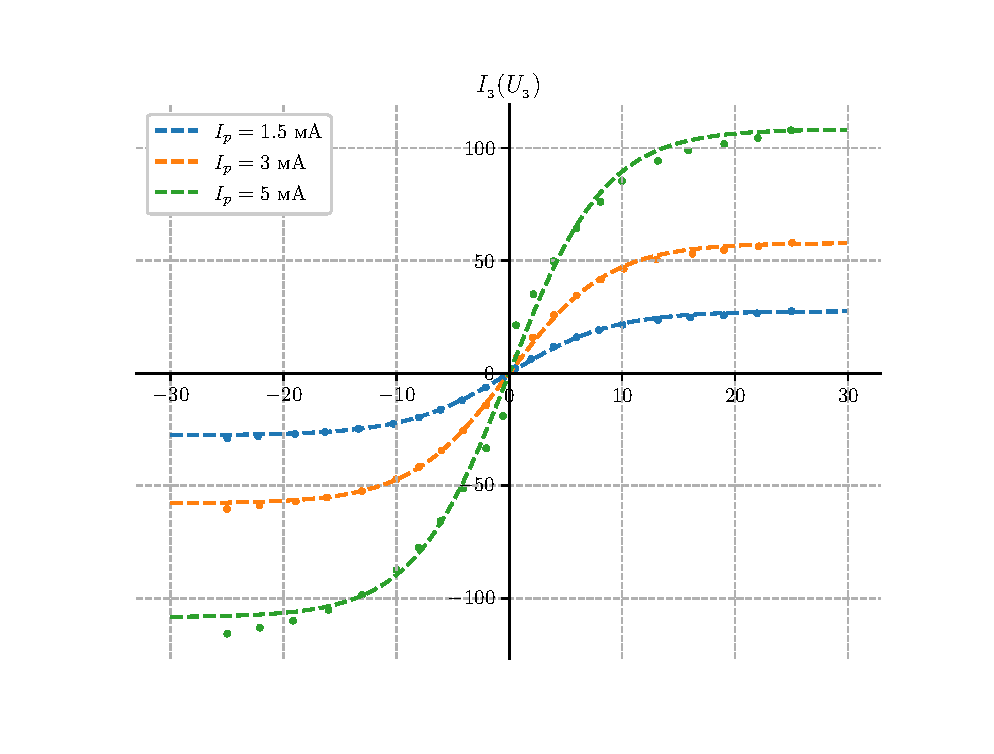
\includegraphics[width=0.7\linewidth]{pics/all.eps}
    \caption{ВАХ двойного зонда при различных токах}
\end{figure}
Как видно из графиков, ионный ток насыщения различен для половин графиков выше и ниже нуля, поэтому будем брать его усредненное значение.

$I_{iн}(5мА) = 88.0 \pm 4.7$ мкА, $I_{iн}(3мА) = 45.1 \pm 1.0$ мкА, $I_{iн}(1.5мА) = 20.3 \pm 0.5$ мкА

% $\dfrac{dI}{dU}|_{U=0}(5мА) = (2.87\pm 0.03) \cdot 10^{-8} А/В$,\quad $\dfrac{dI}{dU}|_{U=0}(3мА) = (1.1\pm 0.2) \cdot 10^{-7} А/В$,

% $\dfrac{dI}{dU}|_{U=0}(1.5мА) = (2.7\pm 0.3) \cdot 10^{-7} А/В$, 
 
% Теперь можем из (12) вычислить температуру электронов $T_e = (1.8 \pm 0.1) \cdot 10^7$ К, $(2.4 \pm 0.5) \cdot 10^6$ К и $(4.4 \pm 0.6) \cdot 10^5$ К соответсвенно.

Теперь из (12) можем вычислить температуру электронов $T_e$.
% $T_e = (1.7 \pm 0.1) \cdot 10^4$ К, $T_e = (2.4 \pm 0.5) \cdot 10^4$ К, $T_e = (3.9 \pm 0.1) \cdot 10^4$ К соответсвенно.
% \vspace{0.3cm}

Также из (7) расчитаем концентрацию ионов $n_i$, полагая ее равной концентрации электронов $n_e$.
% $n_e = (6.0 \pm 0.5) \cdot 10^{13} м^{-3}$, $n_e = (2.6 \pm 0.3) \cdot 10^{13} м^{-3}$, $n_e = (9.1 \pm 0.3) \cdot 10^{12} м^{-3}$.
% \vspace{0.3cm}

Из (5) получим плазменную частоту колебаний электронов $\omega_p$
% = (4.6 \pm 0.2)\cdot 10^3 {рад \over с}$, $\omega_p = (3.0 \pm 0.2)\cdot 10^3 {рад \over с}$, $\omega_p = (1.8 \pm 0.1)\cdot 10^3 {рад \over с}$.
% \vspace{0.3cm}

Расчитаем электронную поляризационную длину $r_{D_e}$, радиус Дебая $r_{D}$ и по формуле (4)  вычислим среднее число ионов в сфере такого радиуса $<N_D>$.
% $r_{D_e} = (1.5 \pm) \cdot 10^{-4}$ м, $r_{D_e} = (1.5 \pm) \cdot 10^{-4}$ м
Степень ионизации $\alpha$ получим по соотношению $\alpha = n_i/n$, где $n$ -- общее число частиц в единице объема (давление $P=nkT_i\approx 1$мбар). 
Все результаты занесем в таблицу 3.
\begin{table}[H]
    \centering
    \resizebox{\textwidth}{!}{
    \begin{tabular}[]{|c|c|c|c|c|c|c|c|}
        \hline 
        $I_p$, мА&$T_e, 10^4$, К&$n_e, 10^{13} м^{-3}$&$\omega_p, 10^3{рад \over сек}$&$r_{D_e}, 10^{-4}м$&$r_D, 10^{-4}$&$<N_D>, 10^3$&$\alpha, 10^{-6}$\\
        \hline
        5&$1.7\pm 0.1$ &$6.0 \pm 0.5$&$4.6\pm0.2$&$3.4\pm0.2$&$1.5\pm0.1$&$0.85\pm0.24$&$14\pm2$\\
        \hline
        3&$2.4\pm 0.5$ &$2.6 \pm 0.3$&$3.0\pm0.2$&$6.2\pm0.5$&$2.2\pm0.1$&$1.2\pm0.3$&$8.6\pm0.7$\\
        \hline
        1.5&$3.9\pm 0.1$&$0.91 \pm0.03$&$1.8\pm0.1$&$13.5\pm0.4$&$3.8\pm0.1$&$2.1\pm0.3$&$4.9\pm0.3$\\
        \hline
    \end{tabular}}
    \caption{Вычисленные характеристики}
\end{table}

\subsection*{Подведение итогов}
В ходе работы снята вольт-амперная характеристика тлеющего разряда и зондовые характеристики при разных токах разряда.
По результатам измерений рассчитаны концентрация и температура электронов в плазме, плазменная частота, поляризационная длина, дебаевский радиус экранирования и степень ионизации.

По полученным значениям характеристик можно заключить, что плазма не является квазинейтральной, т.к. электронная поляризационная длина не сильно превосходит дебаевский радиус.
При этом плазму можно считать идеальным газом, в связи с тем, что число Дебая сильно превосходит единицу.
\end{document}